\chapter{Data} \label{chap:data}
Dataset~\cite{dataset} for the project is X-ray images that collected at Guangzhou Women and Children’s Medical Center, Guangzhou from pediatric patients aged between one to five.
All X-ray images are in JPEG format and organized into folder based structure.
Main sub-structures in the dataset are train, validation and the test folders.
All main folders also broken into sub-folders that named \emph{Normal} and \emph{Pneumonia} to indicate their classification.
All X-rays have graded by expert physicians and check individually, damaged or un-readable X-rays discarded.
Below are the illustrative examples from both classes of the X-ray.

\begin{figure}[H]%
    \centering
    \subfloat[X-ray without Pnuemonia]{{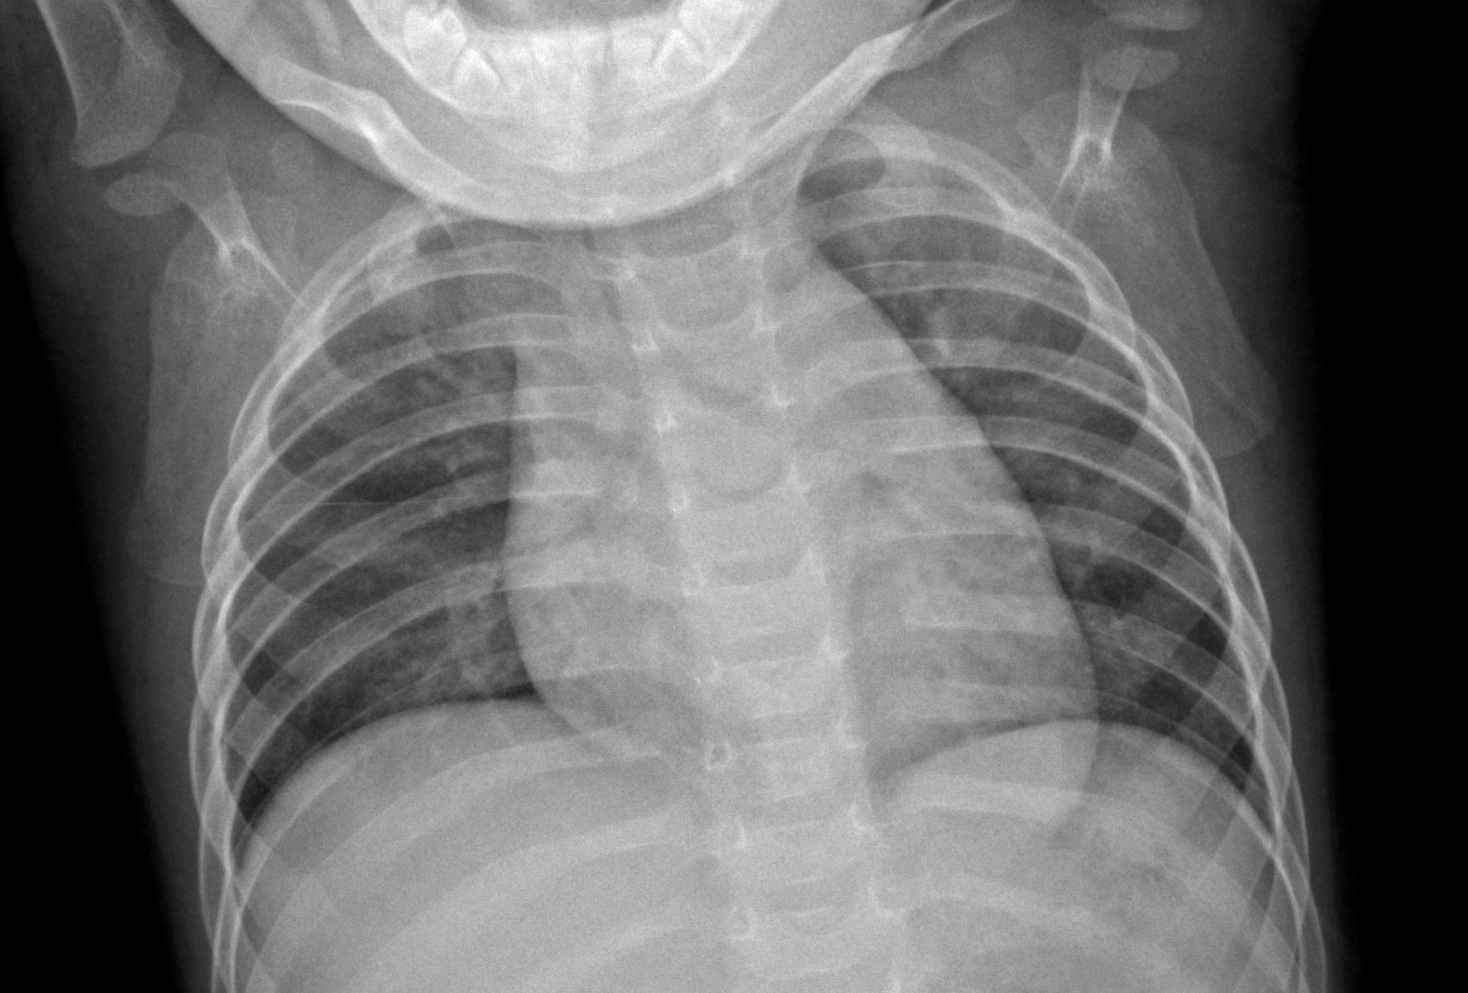
\includegraphics[width=.4\textwidth]{img/chest_xray_train_NORMAL_IM-0133-0001.jpeg} }}%
    \qquad
    \subfloat[X-ray with Pnuemonia]{{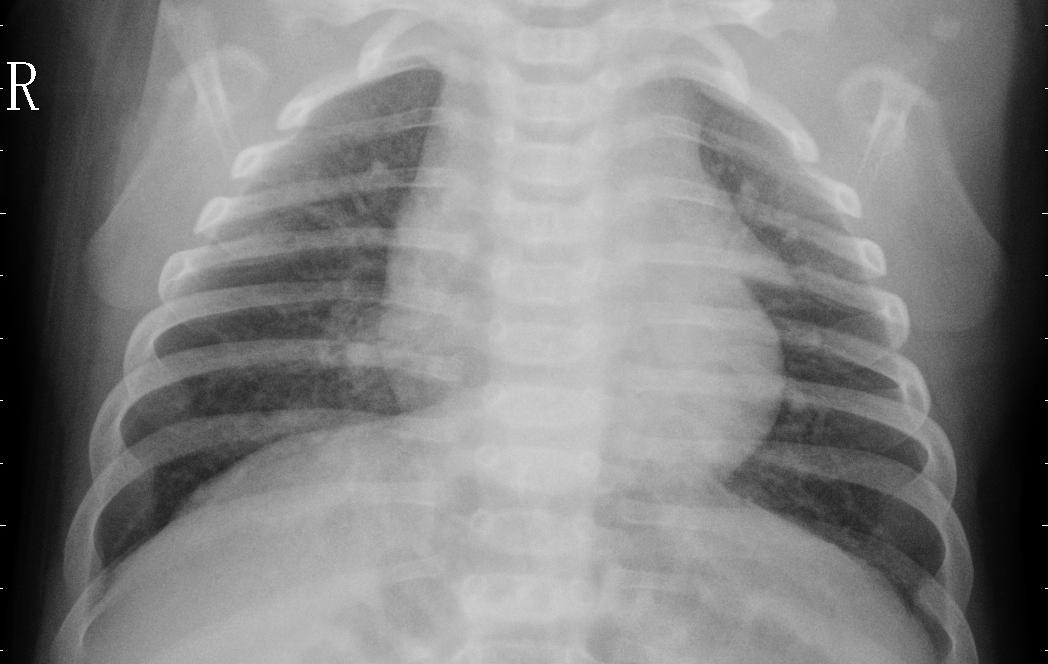
\includegraphics[width=.4\textwidth]{img/chest_xray_train_PNEUMONIA_person1007_virus_1690.jpeg} }}%
    \caption{Two sample X-ray Chest images with and without pneumonia.}%
    \label{fig:sample}%
\end{figure}

For more detailed understanding of the data, I have checked the content of the each train, validation and test datasets. 
There is a significant imbalance in between Pneumonia and Normal classes for train and the test datasets.
Detailed breakdown of each dataset is given in the table \ref{table:dataset}.


\begin{table}[H]
    \centering
    \begin{tabular}{||c c c c||} 
    \hline
    Dataset Name & No of images & Pneumonia & Normal \\ [0.5ex] 
    \hline\hline
    Train & 5216 & 3875 & 1341 \\ 
    \hline
    Validation & 16 & 8 & 8 \\
    \hline
    Test & 624 & 390 & 234 \\ [1ex] 
    \hline
    \end{tabular}
    \caption{Breakdown of images for each classification folder}
    \label{table:dataset}
\end{table}



\section{Data Augmentation}
Data augmentation is a process of producing additional training instances by modifying existing training data points.
Process of data argumentation is very common within the computer vision field.
Generally because it is well understood that the images could be modified some way without having tp loose the classification of the image.
For example image of a cat on the table can be cropped such a way that will still contain the cat on the table but without the background that is not relevant.
Resulting image from this cropping will also be an image classified as a cat image.

There are similarity set of transformation that could be applied to images to create labelled data instances. 
It is import to choose which augmentation to apply and which one to abandon.
Example to highlight some argumentation that is not appropriate is flipping image upside down. 
Even though flipping upside down is acceptable some cases like the cat image example we considered earlier. 
It would not be useful in the setting of Pneumonia classification because considering upside down X-rays is not natural occurrence in the field of medical diagnosis.
Perhaps most striking example of area that this argumentation technique should not be used is hand written digits classification. 
Reason for that is although upside number one is still an image of number one, in the case for number six it will result images labelled as six but in content they will appear as number nine. 
Train machine learning model with samples of number nine labelled as six will indeed hinder the accurate of the model instead of helping it.

\begin{figure}[H]
    \centering
    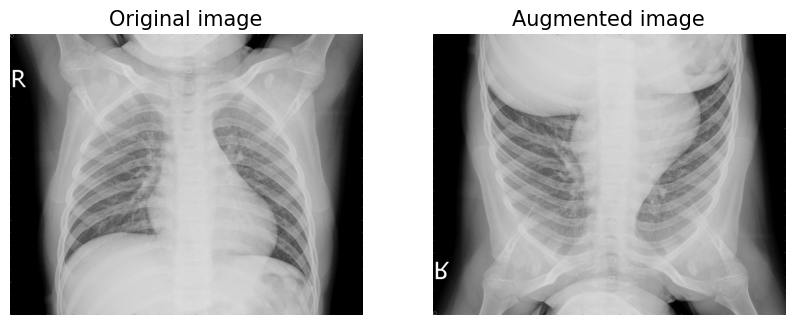
\includegraphics[width=\textwidth]{img/augmented-image-1588951790.png}
    \caption{Flipping an image upside down is not applied in CAD context}
    \label{fig:upsidedownxray}
  \end{figure}


Data augmentations applied and example results of the augmentation.

\section{Limitations of the Dataset}
Issues related to validation set size. Variance of the image resolution.

\section{Data Procession}
Information about tf.data processing pipeline and advantages compare to other data feeds.

Information about data processing for scikit-learn models.
Talk about the decisions for image size and how it relates to information loss and preservation. Briefly mention the high variance of the image sizes and image resizing options and choice.
Discussing different representation of the dataset will be covered.
Talk about data module design and functionality.
\clearpage